\begin{figure*}%[!htbp]
\begin{center}
\begin{subfigure}[b]{0.6\columnwidth}
  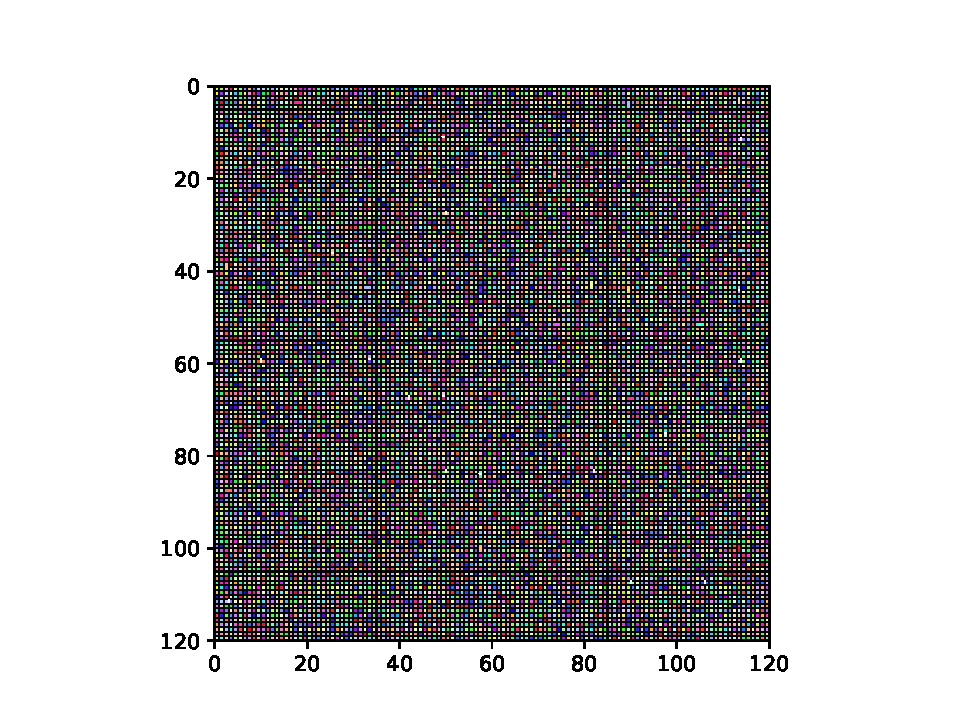
\includegraphics[width=\columnwidth,trim={2.5cm 0.5cm 2.5cm 1cm},clip]{img/ChannelMap_1011_update0}
  \caption{Update 0; gen. 0}
  \label{fig:ChannelMap_1011_update0}
\end{subfigure}%
\begin{subfigure}[b]{0.6\columnwidth}
  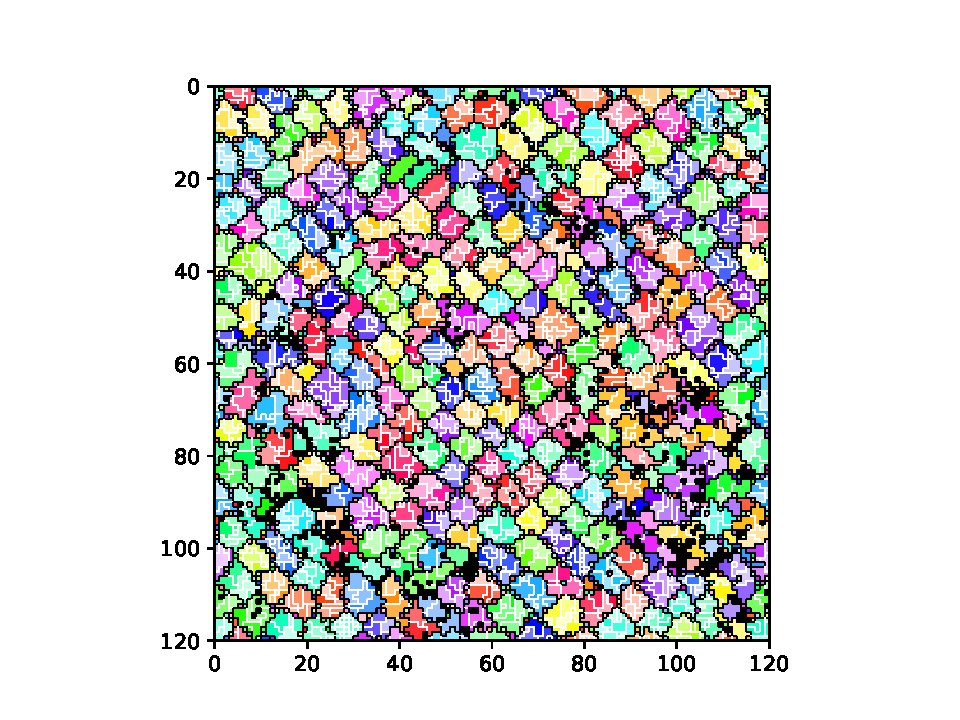
\includegraphics[width=\columnwidth,trim={2.5cm 0.5cm 2.5cm 1cm},clip]{img/ChannelMap_1011_update1000000}
  \caption{Update 1M; gen. 927}
  \label{fig:ChannelMap_1011_update1000000}
\end{subfigure}%
\begin{subfigure}[b]{0.6\columnwidth}
  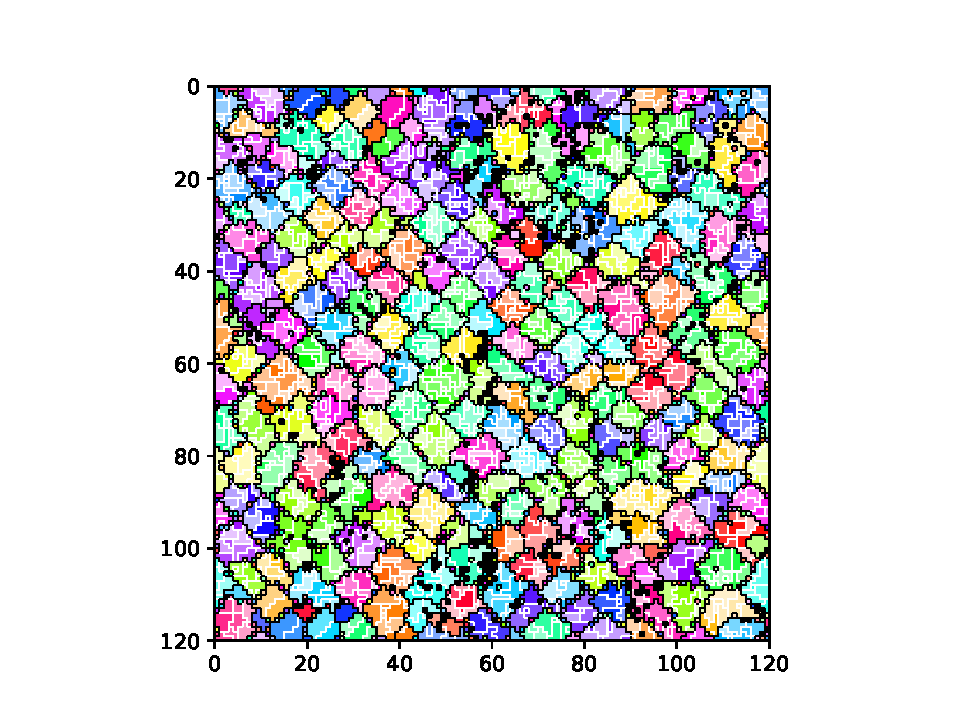
\includegraphics[width=\columnwidth,trim={2.5cm 0.5cm 2.5cm 1cm},clip]{img/ChannelMap_1011_update2000000}
  \caption{Update 2M; gen. 1,917}
  \label{fig:ChannelMap_1011_update2000000}
\end{subfigure}
\begin{subfigure}[b]{0.6\columnwidth}
  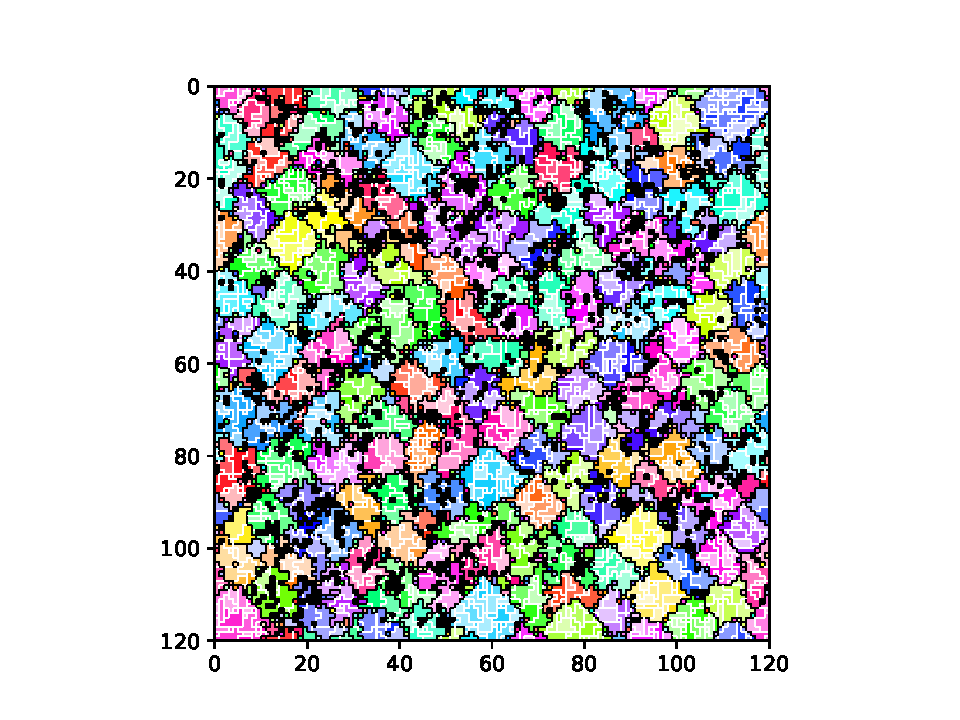
\includegraphics[width=\columnwidth,trim={2.5cm 0.5cm 2.5cm 1cm},clip]{img/ChannelMap_1011_update4000000}
  \caption{Update 4M; gen. 4,053}
  \label{fig:ChannelMap_1011_update4000000}
\end{subfigure}%
\begin{subfigure}[b]{0.6\columnwidth}
  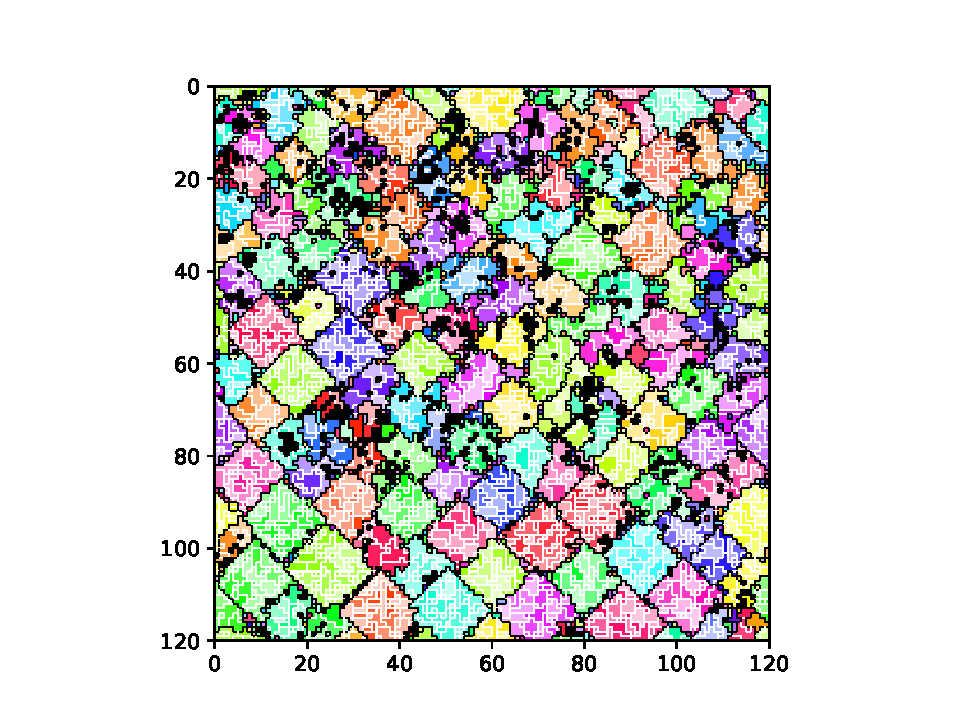
\includegraphics[width=\columnwidth,trim={2.5cm 0.5cm 2.5cm 1cm},clip]{img/ChannelMap_1011_update5000000}
  \caption{Update 5M; gen. 5,173}
  \label{fig:ChannelMap_1011_update5000000}
\end{subfigure}%
\begin{subfigure}[b]{0.6\columnwidth}
  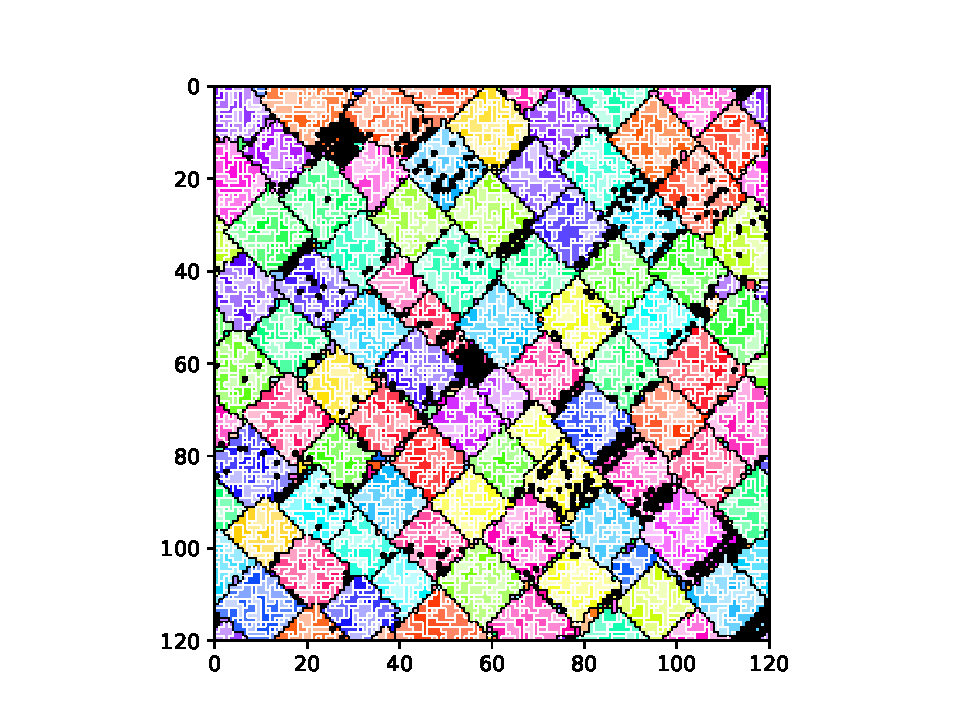
\includegraphics[width=\columnwidth,trim={2.5cm 0.5cm 2.5cm 1cm},clip]{img/ChannelMap_1011_update7000000}
  \caption{Update 7M; gen. 7,312}
  \label{fig:ChannelMap_1011_update7000000}
\end{subfigure}
\caption{
Progression of of same-channel level-one and level-two signaling networks states in an evolutionary run where second-level individuality evolved.
Level-one channels are coded by color saturation and level-two channels are coded by color hue.
A single cell-like organism occupies each grid tile except for black tiles, which are empty.
}
\label{fig:grid_progression}
\end{center}
\end{figure*}
